\section{Control Structures}



\begin{concept}{Control Structure Types}\\
Three fundamental types of control structures:

\textbf{1. Sequence}:
\begin{itemize}
  \item Linear execution of instructions
  \item No branching or decisions
  \item Operations performed in order
\end{itemize}

\textbf{2. Selection}:
\begin{itemize}
  \item Conditional execution (if-then-else)
  \item Branch based on condition
  \item Different paths based on test
\end{itemize}

\textbf{3. Iteration}:
\begin{itemize}
  \item Repeated execution (loops)
  \item Condition-controlled repetition
  \item Fixed number of repetitions
\end{itemize}

Program flow can be represented with three elements:

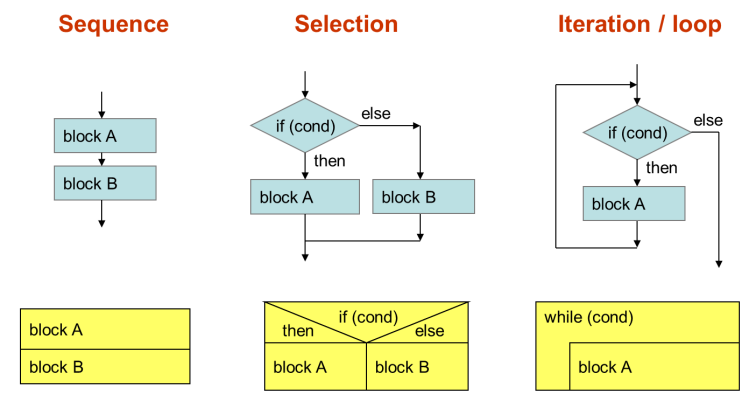
\includegraphics[width=\linewidth]{images/tyoesofcontrolstructures.png}

\begin{itemize}
    \item High level programming language provides these control structures
    \item Compiler translates control structures to assembly using conditional
    and unconditional jumps
\end{itemize}
\end{concept}

\begin{KR}{Implementing Control Structures}\\
Steps for implementing control structures:
\begin{enumerate}
  \item Choose appropriate control structure:
    \begin{itemize}
      \item If-then-else for simple decisions
      \item Switch for multiple cases with same variable
      \item Loops for repeated operations
    \end{itemize}
  \item For switches:
    \begin{itemize}
      \item Create jump table
      \item Calculate offset based on case value
      \item Handle default case
    \end{itemize}
  \item For loops:
    \begin{itemize}
      \item Initialize counter/condition
      \item Place condition check appropriately
      \item Ensure proper exit condition
      \item Update variables correctly
    \end{itemize}
\end{enumerate}
\end{KR}

\begin{remark}
Important considerations:
\begin{itemize}
  \item Consider branch range limitations
  \item Be aware of condition flag changes
  \item Handle corner cases in comparisons
  \item Plan for proper loop termination
  \item Document complex branching logic
\end{itemize}
\end{remark}

\columnbreak


\subsubsection{Selection Structures}


\begin{definition}{IF-ELSE}
    Compiler translates \textbf{selection} into assembly code using conditional and unconditional jumps:\\
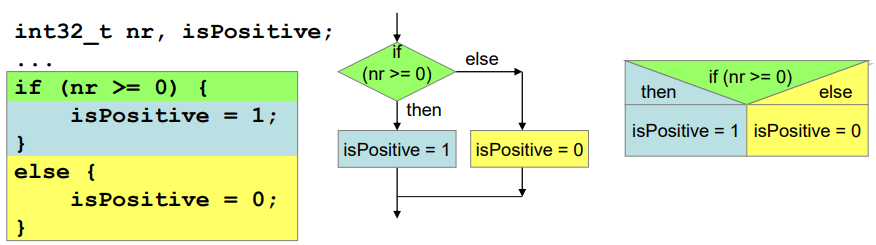
\includegraphics[width=\linewidth]{images/ifelse1.png}

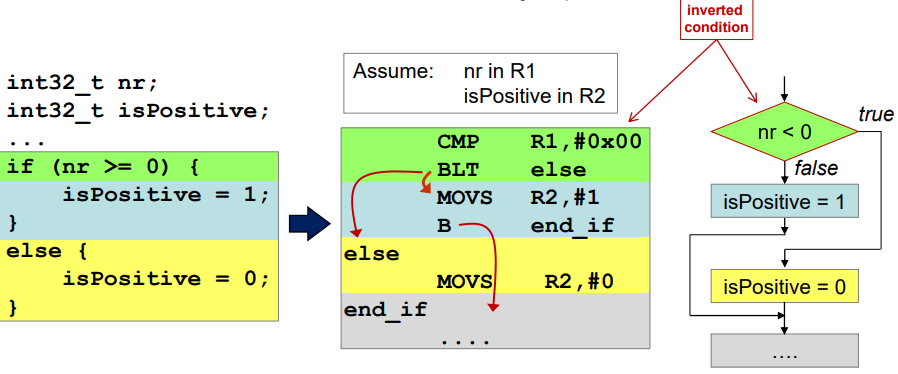
\includegraphics[width=\linewidth]{images/ifelse2.png}
\end{definition}

\begin{KR}{Selection Implementation}

1. Simple if-then:
\begin{lstlisting}[language=armasm, style=basesmol]
    ; if (x > 0) { x++; }
    CMP     R0, #0          ; Compare x with 0
    BLE     endif           ; Skip if x <= 0
    ADDS    R0, #1          ; x++
endif
\end{lstlisting}

2. if-then-else:
\begin{lstlisting}[language=C, style=basesmol]
    if (condition) {    //then-part
    } else {            //else-part
    }
\end{lstlisting}
\vspace{-4mm}
\begin{lstlisting}[language=armasm, style=basesmol]
    CMP     R0, #value      ; Test condition
    BNE     else_part       ; Branch if false
then_part
    ; Then code
    B       endif           ; Skip else
else_part
    ; Else code
endif
    ; Continue execution
\end{lstlisting}

3. Nested if:
\begin{lstlisting}[language=C, style=basesmol]
    if (x > 0) {
        if (y > 0) {
            x = y;
        }
    }
\end{lstlisting}
\vspace{-4mm}
\begin{lstlisting}[language=armasm, style=basesmol]
    CMP     R0, #0          ; Check x > 0
    BLE     endif_outer
    CMP     R1, #0          ; Check y > 0
    BLE     endif_inner
    MOVS    R0, R1          ; x = y
endif_inner
endif_outer
\end{lstlisting}
\end{KR}

\begin{KR}{Selection Implementation} with multiple Conditions

1. Multiple conditions (AND):
\begin{lstlisting}[language=C, style=basesmol]
if (condA && condB) {   //then-part
} else {                //else-part
}
\end{lstlisting}
\vspace{-4mm}
\begin{lstlisting}[language=armasm, style=basesmol]
    ; Test first condition
    CMP     Rx, #valA
    B<cc>   else_label        ; Branch if first fails
    ; Test second condition
    CMP     Ry, #valB
    B<cc>   else_label        ; Branch if second fails

    ; Then part
    <then instructions>
    B       endif_label
    
else_label
    ; Else part
    <else instructions>
    
endif_label
\end{lstlisting}

2. Multiple conditions (OR):
\begin{lstlisting}[language=C, style=basesmol]
if (condA || condB) {   //then-part
} else {                //else-part
}
\end{lstlisting}
\vspace{-4mm}
\begin{lstlisting}[language=armasm, style=basesmol]
    ; Test first condition
    CMP     Rx, #valA
    B<cc>   test_second       ; Try second if first fails
    B       then_label        ; First succeeded
    
test_second
    CMP     Ry, #valB
    B<cc>   else_label        ; Branch if both fail
    
then_label
    ; Then part
    <then instructions>
    B       endif_label
    
else_label
    ; Else part
    <else instructions>
    
endif_label
\end{lstlisting}
\end{KR}

\begin{theorem}{Limitations of Conditional Branches}\\
    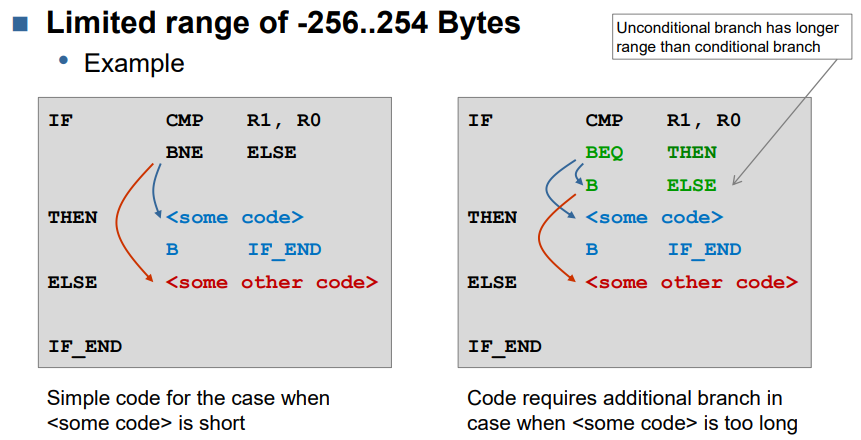
\includegraphics[width=\linewidth]{images/limitsofconditionalbranches.png}
\end{theorem}

\columnbreak

\begin{definition}{Switch-Case}\\
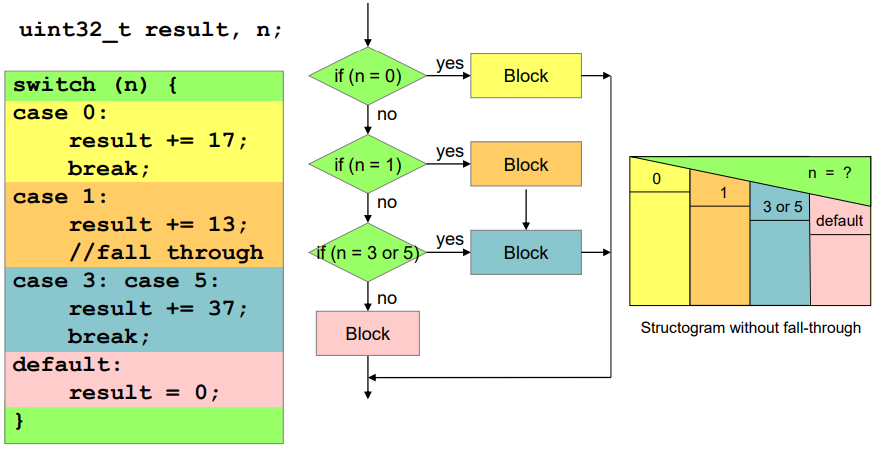
\includegraphics[width=\linewidth]{images/switchcases.png}\\
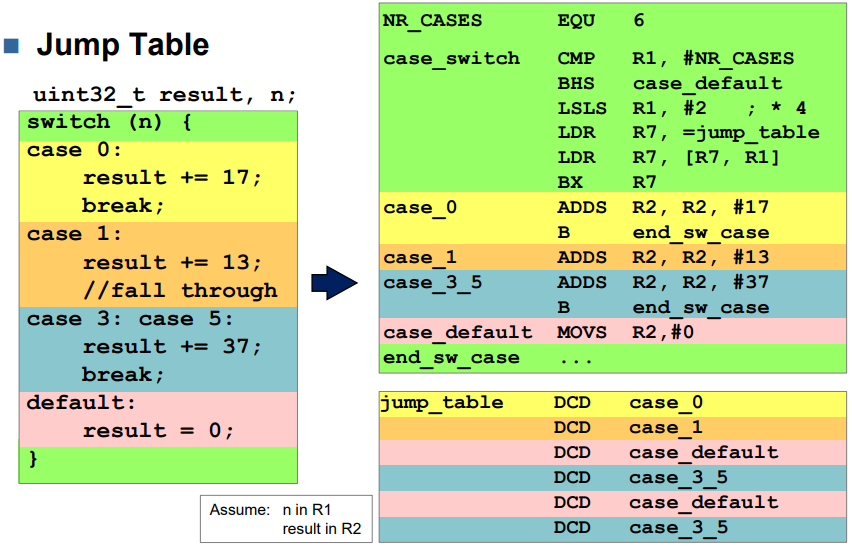
\includegraphics[width=0.9\linewidth]{images/switchcases2.png}
\end{definition}

\begin{KR}{Switch Implementation}

1. Range check and table access:
\begin{lstlisting}[language=armasm, style=basesmol]
    CMP     R0, #MAX_CASES  ; Check range
    BHS     default_case    ; If too high, default
    LSLS    R0, #2          ; Multiply by 4
    LDR     R1, =jump_table ; Load table address
    ADD     R1, R0          ; Add offset
    LDR     R1, [R1]        ; Load target address
    BX      R1              ; Branch to case
\end{lstlisting}

2. Jump table structure:
\begin{lstlisting}[language=armasm, style=basesmol]
jump_table
    DCD     case_0          ; Case 0 handler
    DCD     case_1          ; Case 1 handler
    DCD     default_case    ; Default handler
    ; ... more cases
\end{lstlisting}

3. Case handlers:
\begin{lstlisting}[language=armasm, style=basesmol]
case_0
    ; Handle case 0
    B       switch_end
case_1
    ; Handle case 1
    B       switch_end
default_case
    ; Handle default case
switch_end
\end{lstlisting}
\end{KR}



\begin{example2}{Switch Statement Implementation}
C code example:
\begin{lstlisting}[language=C, style=basesmol]
uint32_t result, n;
switch (n) {
    case 0:
        result += 17;
        break;
    case 1:
        result += 13;
        //fall through
    case 3: 
    case 5:
        result += 37;
        break;
    default:
        result = 0;
}
\end{lstlisting}

Assembly implementation with jump table:
\begin{lstlisting}[language=armasm, style=basesmol]
NR_CASES    EQU     6
case_switch CMP     R1, #NR_CASES
            BHS     case_default
            LSLS    R1, #2        ; * 4
            LDR     R7, =jump_table
            LDR     R7, [R7, R1]
            BX      R7

case_0      ADDS    R2, R2, #17
            B       end_sw_case
case_1      ADDS    R2, R2, #13
case_3_5    ADDS    R2, R2, #37
            B       end_sw_case
case_default MOVS   R2, #0
end_sw_case ...

jump_table  DCD     case_0
            DCD     case_1
            DCD     case_default
            DCD     case_3_5
            DCD     case_default
            DCD     case_3_5
\end{lstlisting}
\end{example2}

\pagebreak

\subsubsection{Loops}

\begin{concept}{Do-While (Post-Test Loop)}:
Compiler translates \textbf{post-test} loops into assembly code using conditional branches:\\
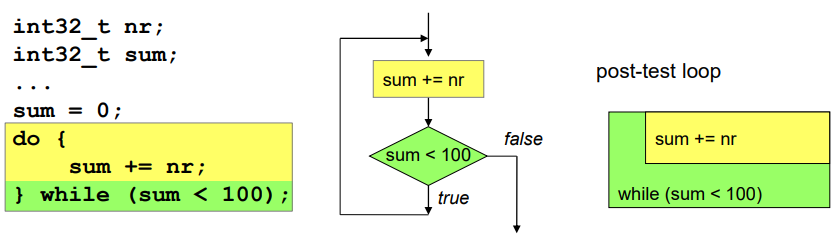
\includegraphics[width=\linewidth]{images/dowhile.png}\\
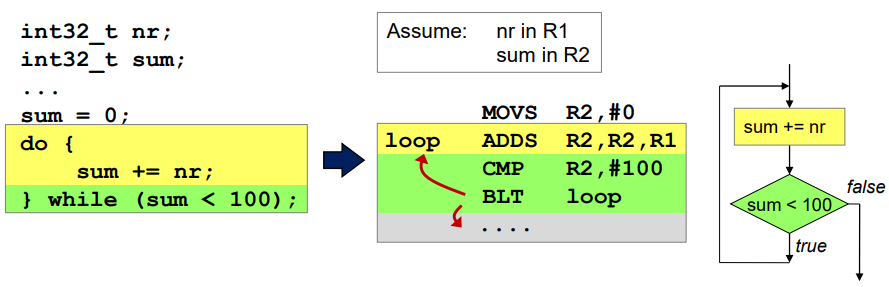
\includegraphics[width=\linewidth]{images/dowhile2.png}
\end{concept}

\begin{KR}{Do-While loop}
\begin{lstlisting}[language=armasm, style=basesmol]
    ; do { x++; } while (x < 10);
do_loop
    ADDS    R0, #1          ; x++
    CMP     R0, #10         ; Check x < 10
    BLT     do_loop         ; Continue if true
\end{lstlisting}
\end{KR}

\begin{concept}{While (Pre-Test Loop)}:
Compiler translates \textbf{pre-test} loops into assembly code reusing structure of do-while:\\
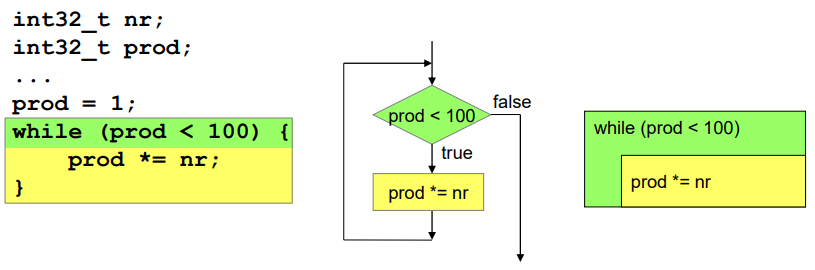
\includegraphics[width=\linewidth]{images/whileloop.png}\\
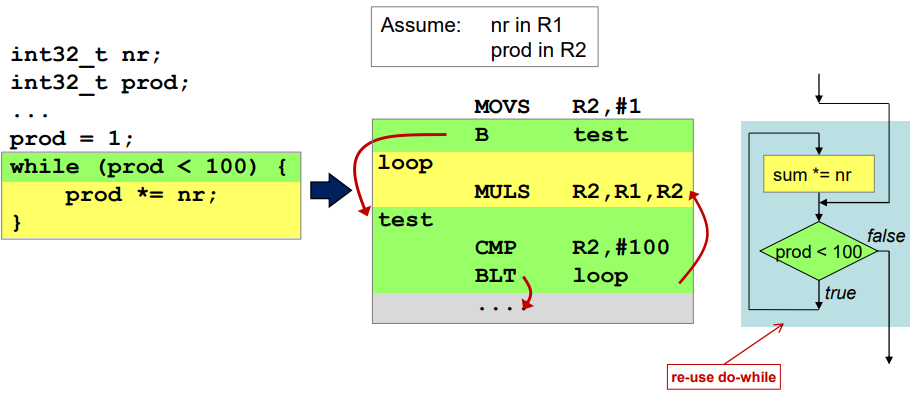
\includegraphics[width=\linewidth]{images/whileloop2.png}
\end{concept}

\begin{KR}{While loop}
\begin{lstlisting}[language=armasm, style=basesmol]
    ; while (x < 10) { x++; }
    B       while_cond      ; Jump to condition
while_loop
    ADDS    R0, #1          ; x++
while_cond
    CMP     R0, #10         ; Check x < 10
    BLT     while_loop      ; Continue if true
\end{lstlisting}
\end{KR}

\begin{concept}{For Loop (Pre-Test Loop)}:\\
For-Loops are converted into while-loops by the compiler.\\
break and continue statements require special treatment.\\
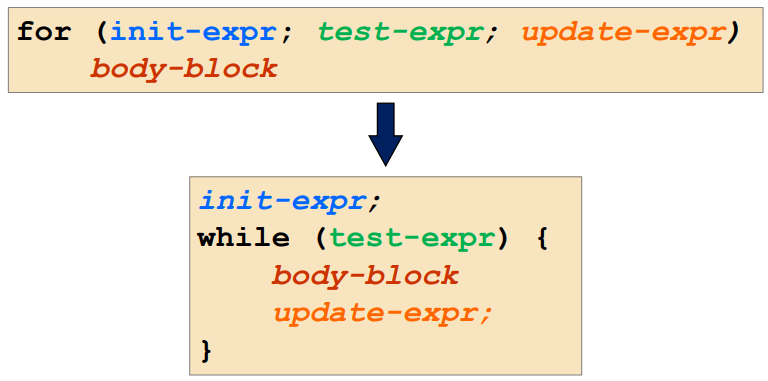
\includegraphics[width=\linewidth]{images/forloop.png}
\end{concept}


\begin{KR}{For loop}
\begin{lstlisting}[language=armasm, style=basesmol]
    ; for (i = 0; i < 10; i++)
    MOVS    R0, #0          ; i = 0
    B       for_cond
for_loop
    ; Loop body
    ADDS    R0, #1          ; i++
for_cond
    CMP     R0, #10         ; Check i < 10
    BLT     for_loop        ; Continue if true
\end{lstlisting}
\end{KR}



\begin{example2}{Complex Control Structure}\\
Implementing nested loops with conditions:

\begin{lstlisting}[language=C, style=basesmol]
for (i = 0; i < 5; i++) {
    if (i == 2) continue;
    for (j = 0; j < 3; j++) {
        if (j == 1) break;
        sum += i + j;
    }
}
\end{lstlisting}
\begin{lstlisting}[language=armasm, style=basesmol]
    MOVS    R0, #0          ; i = 0
outer_loop
    CMP     R0, #2          ; Check i == 2
    BEQ     outer_continue  ; Skip if i == 2
    
    MOVS    R1, #0          ; j = 0
inner_loop
    CMP     R1, #1          ; Check j == 1
    BEQ     outer_continue  ; Break to outer loop
    
    ADDS    R2, R0, R1      ; Calculate i + j
    ADDS    R4, R4, R2      ; Add to sum
    
    ADDS    R1, #1          ; j++
    CMP     R1, #3          ; Check j < 3
    BLT     inner_loop      ; Continue inner loop
    
outer_continue
    ADDS    R0, #1          ; i++
    CMP     R0, #5          ; Check i < 5
    BLT     outer_loop      ; Continue outer loop
\end{lstlisting}
\end{example2}

\subsubsection{String Processing}

\begin{KR}{String Processing Patterns}\\
Common patterns for string manipulation:

1. String traversal:
\begin{lstlisting}[language=armasm, style=basesmol]
    MOVS    R2, #0          ; Index
loop
    LDRB    R3, [R0, R2]    ; Load char
    CMP     R3, #0          ; Check end
    BEQ     done            ; Exit if terminator
    ; Process character
    ADDS    R2, R2, #1      ; Next char
    B       loop
\end{lstlisting}

2. Character transformation:
\begin{lstlisting}[language=armasm, style=basesmol]
    ; Check character range
    CMP     R3, #lower_bound
    BLO     skip            ; Below range
    CMP     R3, #upper_bound
    BHI     skip            ; Above range
    
    ; Transform character
    ADDS    R3, #offset     ; Apply offset
    
skip
    STRB    R3, [R1, R2]    ; Store result
\end{lstlisting}

3. String copy:
\begin{lstlisting}[language=armasm, style=basesmol]
    MOVS    R2, #0          ; Index
copy_loop
    LDRB    R3, [R0, R2]    ; Load source
    STRB    R3, [R1, R2]    ; Store to dest
    ADDS    R2, R2, #1      ; Next char
    CMP     R3, #0          ; Check end
    BNE     copy_loop       ; Continue if not done
\end{lstlisting}
\end{KR}

\begin{remark}
Important considerations:
\begin{itemize}
  \item Choose appropriate conditional branches
  \item Consider signed vs unsigned comparisons
  \item Handle edge cases and termination
  \item Maintain proper register allocation
  \item Document complex control flow
\end{itemize}
\end{remark}

\begin{example2}{String Processing Loop}\\
Converting string to uppercase:
\begin{lstlisting}[language=armasm, style=basesmol]
    AREA    progCode, CODE, READONLY
    THUMB
main
    PROC
    EXPORT  main
    LDR     R0, =srcstr     ; Source string
    LDR     R1, =outstr     ; Output string
    MOVS    R2, #0          ; Initialize index
    
cond
    LDRB    R3, [R0, R2]    ; Load character
    CMP     R3, #0          ; Check for end
    BEQ     endloop         ; Exit if done
    CMP     R3, #60         ; Check if < 'a'
    BLO     store           ; Skip if not lowercase
    CMP     R3, #90         ; Check if > 'z'
    BHI     store           ; Skip if not lowercase
    ADDS    R3, R3, #32     ; Convert to uppercase
    
store
    STRB    R3, [R1, R2]    ; Store character
    ADDS    R2, R2, #1      ; Next character
    B       cond            ; Continue loop
    
endloop
    STRB    R3, [R1, R2]    ; Store terminator
    ENDP
    
srcstr  DCB     "This IS mY TestStriNG", 0
    AREA    progData, DATA, READWRITE
outstr  SPACE   50
\end{lstlisting}

\textbf{Structogram:}\\
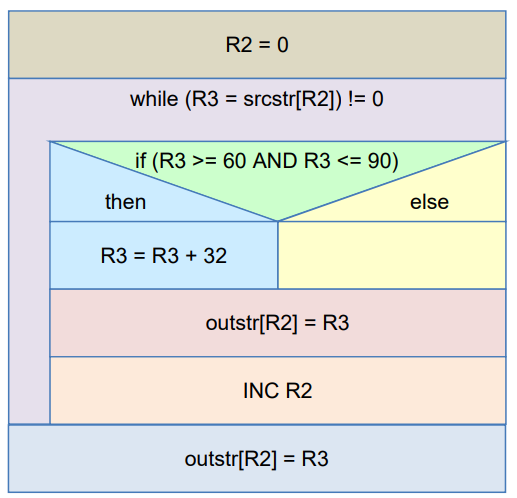
\includegraphics[width=0.8\linewidth]{images/structogramstringstuff.png}

\textbf{Result:} "THIS IS MY TESTSTRING"
\end{example2}